% Branch and bound tree for maximize knapsack
\tikzset{
  S/.style = {draw, rectangle, rounded corners=0.1cm, minimum size = 8mm,  top color=blue!10, bottom color=blue!10},% top color=white, bottom color=blue!20},
}
     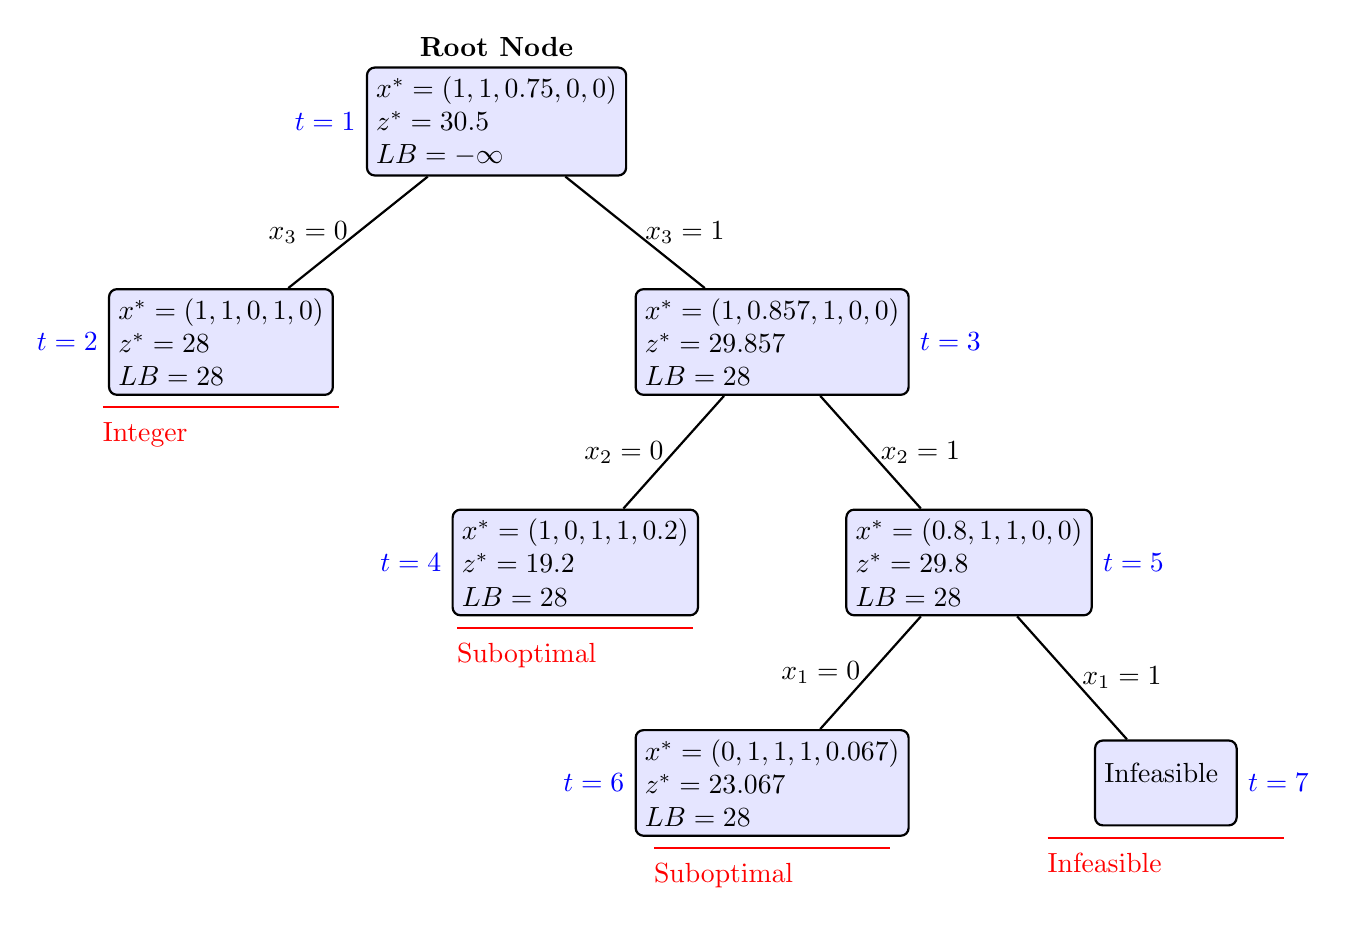
\begin{tikzpicture}[-,thick]
\node[S,sibling distance=5cm, level distance=1.3cm, align=left, label={[blue]left:$t = 1$}, label = {above:\textbf{Root Node}}] 
	{$x^* = (1,1,0.75,0,0) $\\ $z^* = 30.5$\\ $ LB = -\infty$} 
	[sibling distance=7cm, level distance=2.8cm,align=left]
	%
     	child {node[S, label={[blue]left:$t = 2$}, label = {[red]below: \rule{3cm}{0.8pt} \\ \centering Integer}] 
     		{$x^* = (1,1,0,1,0) $\\$z^* = 28$\\$ LB = 28$}
		[sibling distance=2.5cm, level distance=2.8cm,align=left]
   		edge from parent node[left] {$x_3 = 0$}
   }
     child {node[S, label={[blue]right:$t =3$}] 
     		{$x^* = (1,0.857,1,0,0) $\\$z^* = 29.857$\\$ LB = 28$}
		[sibling distance=5cm, level distance=2.8cm,align=left]
		%
     		child {node[S, label={[blue]left:$t = 4$}, label = {[red]below: \rule{3cm}{0.8pt} \\ \centering Suboptimal}] {$x^* = (1,0,1,1,0.2)$\\$z^* = 19.2$\\$ LB = 28$}
     			edge from parent node[left] {$x_2 = 0$}}
     		child {node[S, label={[blue]right:$t =5$}] {$x^* = (0.8,1,1,0,0)$\\$z^* = 29.8$\\$ LB = 28$}[sibling distance=5cm, level distance=2.8cm,align=left]
			child {node[S, label={[blue]left:$t =6$}, , label = {[red]below: \rule{3cm}{0.8pt} \\ \centering Suboptimal}] {$x^* = (0,1,1,1,0.067)$\\$z^* = 23.067$\\$ LB = 28$}[sibling distance=5cm, level distance=2.8cm,align=left]
				edge from parent node[left] {$x_1 = 0$}
				}
			child {node[S, label={[blue]right:$t =7$}, label = {[red]below: \rule{3cm}{0.8pt} \\ \centering Infeasible}] {\\ Infeasible \hspace{3cm} \\ }[sibling distance=5cm, level distance=2.8cm,align=left]
				edge from parent node[right] {$x_1 = 1$}
				}
     			edge from parent node[right] {$x_2 = 1$}
			}
   		edge from parent node[right] {$x_3 = 1$}
   };

     \end{tikzpicture}
